% !BIB TS-program = biber

\RequirePackage[l2tabu,orthodox]{nag}

% TODO: decide if one-sided/two-sided
%\documentclass[headsepline,footsepline,footinclude=false,fontsize=11pt,paper=a4,listof=totoc,bibliography=totoc,BCOR=12mm,DIV=12]{scrbook} % two-sided
\documentclass[headsepline,footsepline,footinclude=false,oneside,fontsize=11pt,paper=a4,listof=totoc,bibliography=totoc]{scrbook} % one-sided

% TODO: change citation style in settings
\PassOptionsToPackage{table,svgnames,dvipsnames}{xcolor}

\usepackage[utf8]{inputenc}
\usepackage[T1]{fontenc}
\usepackage[sc]{mathpazo}
\usepackage[ngerman,american]{babel}
\usepackage[autostyle]{csquotes}
\usepackage[%
  backend=biber,
  url=false,
  style=alphabetic,
  maxnames=4,
  minnames=3,
  maxbibnames=99,
  giveninits,
  uniquename=init]{biblatex} % TODO: adapt citation style
\usepackage{graphicx}
\usepackage{scrhack} % necessary for listings package
\usepackage{listings}
\usepackage{lstautogobble}
\usepackage{tikz}
\usepackage{pgfplots}
\usepackage{pgfplotstable}
\usepackage{booktabs}
\usepackage[final]{microtype}
\usepackage{caption}
\usepackage[printonlyused]{acronym}
\usepackage[hidelinks]{hyperref} % hidelinks removes colored boxes around references and links
\AtBeginDocument{%
	\hypersetup{
		pdftitle=\getTitle,
		pdfauthor=\getAuthor,
	}
}
\usepackage{ifthen}

\addto\extrasamerican{
	\def\lstnumberautorefname{Line}
	\def\chapterautorefname{Chapter}
	\def\sectionautorefname{Section}
	\def\subsectionautorefname{Subsection}
	\def\subsubsectionautorefname{Subsubsection}
}

\addto\extrasngerman{
	\def\lstnumberautorefname{Zeile}
}

\bibliography{Bachelor Thesis}

\setkomafont{disposition}{\normalfont\bfseries} % use serif font for headings
\linespread{1.05} % adjust line spread for mathpazo font

% Add table of contents to PDF bookmarks
\BeforeTOCHead[toc]{{\cleardoublepage\pdfbookmark[0]{\contentsname}{toc}}}

% Define TUM corporate design colors
% Taken from http://portal.mytum.de/corporatedesign/index_print/vorlagen/index_farben
\definecolor{TUMBlue}{HTML}{0065BD}
\definecolor{TUMSecondaryBlue}{HTML}{005293}
\definecolor{TUMSecondaryBlue2}{HTML}{003359}
\definecolor{TUMBlack}{HTML}{000000}
\definecolor{TUMWhite}{HTML}{FFFFFF}
\definecolor{TUMDarkGray}{HTML}{333333}
\definecolor{TUMGray}{HTML}{808080}
\definecolor{TUMLightGray}{HTML}{CCCCC6}
\definecolor{TUMAccentGray}{HTML}{DAD7CB}
\definecolor{TUMAccentOrange}{HTML}{E37222}
\definecolor{TUMAccentGreen}{HTML}{A2AD00}
\definecolor{TUMAccentLightBlue}{HTML}{98C6EA}
\definecolor{TUMAccentBlue}{HTML}{64A0C8}

% Settings for pgfplots
\pgfplotsset{compat=newest}
\pgfplotsset{
  % For available color names, see http://www.latextemplates.com/svgnames-colors
  cycle list={TUMBlue\\TUMAccentOrange\\TUMAccentGreen\\TUMSecondaryBlue2\\TUMDarkGray\\},
}

% Settings for lstlistings
\lstset{%
  basicstyle=\ttfamily,
  columns=fullflexible,
  autogobble,
  keywordstyle=\bfseries\color{TUMBlue},
  stringstyle=\color{TUMAccentGreen},
  captionpos=b
}


\newcommand*{\getUniversity}{Technische Universität München}
\newcommand*{\getFaculty}{Department of electrical and computer engineering}
\newcommand*{\getDegree}{B.Sc. Electrical Engineering and Information Technology}
\newcommand*{\getTitle}{Utilisation of ray tracing to improve existing Time-Reversal Algorithms for Microwave Imaging}
\newcommand*{\getAuthor}{Lukas Winklhofer}
\newcommand*{\getSupervisor}{Han Na}
\newcommand*{\getAdvisor}{Prof.\ Dr.-Ing. Thomas Eibert}
\newcommand*{\getSubmissionDate}{Submission date}
\newcommand*{\getSubmissionLocation}{Munich}

\begin{document}

% Set page numbering to avoid "destination with the same identifier has been already used" warning for cover page.
% (see https://en.wikibooks.org/wiki/LaTeX/Hyperlinks#Problems_with_Links_and_Pages).
\pagenumbering{alph}
\begin{titlepage}
  % HACK for two-sided documents: ignore binding correction for cover page.
  % Adapted from Markus Kohm's KOMA-Script titlepage=firstiscover handling.
  % See http://mirrors.ctan.org/macros/latex/contrib/koma-script/scrkernel-title.dtx,
  % \maketitle macro.
  \oddsidemargin=\evensidemargin\relax
  \textwidth=\dimexpr\paperwidth-2\evensidemargin-2in\relax
  \hsize=\textwidth\relax

  \centering

  \IfFileExists{logos/tum.pdf}{%
    
\includegraphics[height=20mm]{logos/tum.pdf}
  }{%
    \vspace*{20mm}
  }

  \vspace{5mm}
  {\huge\MakeUppercase{\getUniversity{}} \par}

  \vspace{5mm}
  {\large\MakeUppercase{\getSchool{}}, \par}
  \vspace{2mm}
  {\large\MakeUppercase{\getDepartment{}} \par}

  \vspace{15mm}
  {\Large \getDegree{} \par}

  \vspace{10mm}
  {\huge\bfseries \getTitle{} \par}

  \vspace{10mm}
  {\LARGE \getAuthor{}}

\end{titlepage}


\frontmatter{}

\begin{titlepage}
  \centering

  \IfFileExists{logos/tum.pdf}{%
    
\includegraphics[height=20mm]{logos/tum.pdf}
  }{%
    \vspace*{20mm}
  }

  \vspace{5mm}
  {\huge\MakeUppercase{\getUniversity{}} \par}

  \vspace{5mm}
  {\large\MakeUppercase{\getSchool{}}, \par}
  \vspace{2mm}
  {\large\MakeUppercase{\getDepartment{}} \par}

  \vspace{20mm}
  {\Large \getDegree{} \par}

  \vspace{15mm}
  {\huge\bfseries \getTitle{} \par}

  \vspace{15mm}
  \begin{tabular}{l l}
    Author:          & \getAuthor{}         \\
    Supervisor:      & \getSupervisor{}     \\
    Advisor:         & \getAdvisor{}        \\
    Submission Date: & \getSubmissionDate{} \\
  \end{tabular}

\end{titlepage}

\thispagestyle{empty}
\vspace*{0.8\textheight}
\noindent
I confirm that this Bachelor thesis is my own work and I have documented all sources and material used.

\vspace{15mm}
\noindent
\getSubmissionLocation{}, \getSubmissionDate{} \hspace{\fill} \getAuthor{}

\cleardoublepage{}

\addcontentsline{toc}{chapter}{Acknowledgments}
\thispagestyle{empty}

\vspace*{20mm}

\begin{center}
    {\usekomafont{sectioning}\usekomafont{section} Acknowledgments}
\end{center}

\vspace{10mm}

I would like to express my sincere thanks to my advisor, Prof.\ Thomas Eibert, for his help and advice. 
I am grateful for his support and for providing me with the opportunity to work on this project.
I would also like to thank my supervisor, Mr.\ Han Na, for his guidance and support throughout the course of this thesis. 
I am grateful for his patience, encouragement, and valuable feedback.
His framework for using the optix ray tracing engine was very helpful and made the implementation of the algorithm much easier. 

\cleardoublepage{}

\chapter{\abstractname}

Imaging algorithms have important applications in our daily life. They are used in medical imaging, security checks, and non-destructive testing. 
A very common algorithm for microwave imaging is the time-reversal algorithm.
This algorithm is often based on full-wave simulations that are computationally expensive.
In this thesis, a new approach to improve time-reversal algorithms for microwave imaging is presented.
To do this the ray concept of the electromagnetic field that arises from geometrical optics is used.
This way the ray-tracing capabilities that are implemented in modern day GPUs can be used to speed up the time-reversal algorithm, especially for complex multipath environments.
The algorithm was implemented using the ray-tracing capabilities of the NVIDIA OptiX framework.
The results show that it can improve the image quality and reduce the computational time compared to the conventional time-reversal algorithm.
For the future work, some ideas are proposed to further improve the algorithm and make it more robust for different scenarios.
For instance the algorithm could be extended to also take the polarization of the electromagnetic field in consideration.
With these improvements the algorithm could be used in real-world applications for example for the localization of wifi routers in a building.

\microtypesetup{protrusion=false}
\tableofcontents{}
\microtypesetup{protrusion=true}

\mainmatter{}

% !TeX root = ../main.tex
% Add the above to each chapter to make compiling the PDF easier in some editors.

\chapter{Introduction}\label{chapter:introduction}

\section{Applications of Microwave Imaging}
Finding information about an area of interest by measuring certain physical properties from this area at one or more places is a fundamental problem.
After all, the human senses (sight, hearing, touch, smell, taste) are all measurements of the environment to recreate a model of the world around us.
Usually the processed information is visualized in a way that is easy to understand for humans, these algorithms are called imaging algorithms.
In electromagnetic (EM) imaging, the goal is to reconstruct the properties of an object from measurements of the scattered electromagnetic field.
This problem is called the inverse-scattering problem.
In some sense our eyes are also an EM imaging system, as they measure the light  which is scattered by the surrounding objects it hits.
The applications of EM-imaging reach from medical imaging (MRI, CT) to security (metal detectors, concealed weapon detection) and geophysics (seismic imaging, ground-penetrating radar).
They vary mostly in the frequency of the used electromagnetic field, as this determines the penetration depth and the resolution of the imaging system.
The higher the frequency, the higher the resolution, but the lower the penetration depth.
This thesis focusses on waves in the microwave frequency range (around 300 MHz to 300 GHz) which corresponds to a wavelength of 1m to 1mm.
Waves of this wavelength will result in a scattering effect when hitting an object of similar size, so they are well suited for practical applications~\parencite{pastorino_microwave_2018}.
Microwave imaging is used in medical applications (breast cancer detection, brain imaging)~\parencite{wang_medical_2014}, security (contraband detection, people screening)~\parencite{ahmed_microwave_2021} and civil engineering (crack detection, subsurface inspection)~\parencite{pastorino_microwave_2018}.

\section{The Principle behind Time-Reversal Imaging}
Time-reversal imaging is about finding the cause of present measurements in the past.
This is can be illustrated by the example of three kids (A, B and C) playing catch with a ball.
Make a video of kid A throwing the ball to kid B and then revert the video.
The video will then show, how the ball flies from kid B to kid A.
Anyone that is asked whether the ball was thrown by kid A or kid C after being shown the reverted video could conclude that it must have been kid A who threw the ball and not kid C.
This problem is trivial if a video of the whole setup and the whole process of throwing and catching the ball is available.
Now suppose, that the video only shows how kid B caught the ball.
Simply time-reverting this video will not reveal who threw the ball in the first place.
But if kid B would exactly replicate the movement in the time-reversed video, it would throw the ball back where it came from so it would land at kid A.
This is the principle behind any time-reversal imaging algorithm.
Its application to microwave imaging is more complex, as the impact of the source doe not spread into one single direction like the ball, but as a wave into all directions.
It shows one of the main flaws of time-reversal imaging, namely that for it to work it is necessary to measure the whole impact of the source.
In case of the player throwing a ball this was easy, as the whole impact is bound to the ball.
A wave on the other hand will propagate in all directions, so there would have to be measurements all around the setting.
Figure~\ref{fig:WaveTimeReversal} shows a receiver array around the source measuring an expanding wave.
The measured signal is then re-emitted by the receivers and contracts at the source location, creating an approximated version of the time-reversed expanding wave (see figure~\ref{fig:WaveTimeReversalContraction}).
If there were infinitely many receivers around the source, they would create a perfect time-reversed wave.

\begin{figure}[ht]
    \centering
    \begin{minipage}{0.45\textwidth}
        \centering
        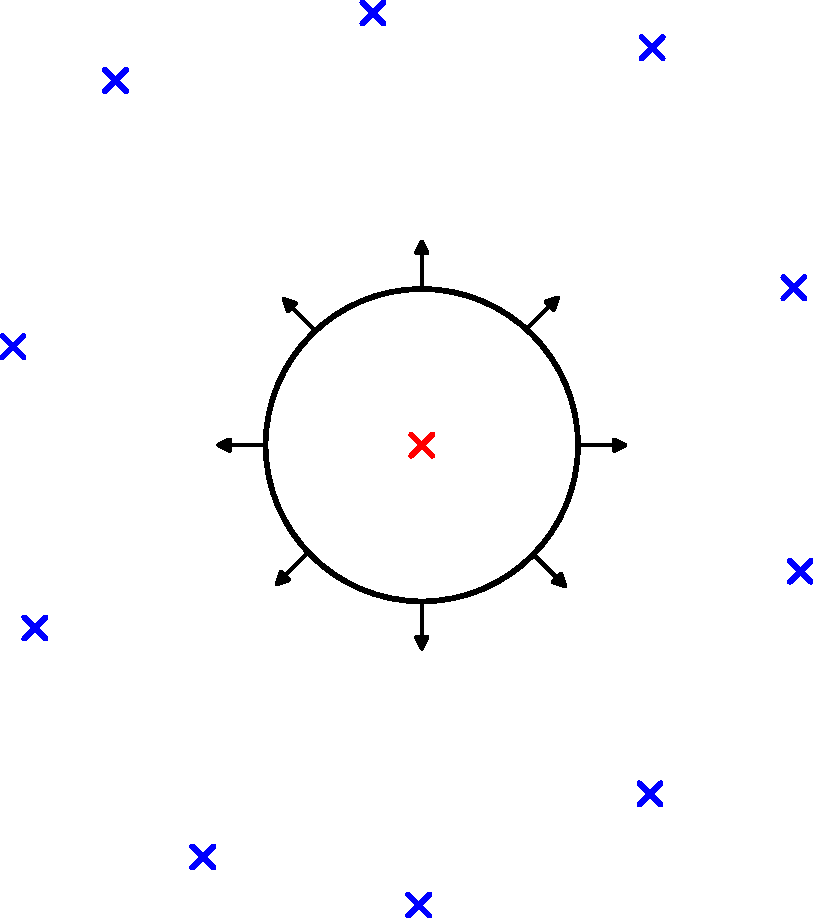
\includegraphics[width=\textwidth]{build/WaveExpanding.pdf}
        \caption{The wave coming from a source (red) is measured at some receivers (blue).}\label{fig:WaveTimeReversal}
    \end{minipage}\hfill
    \begin{minipage}{0.45\textwidth}
        \centering
        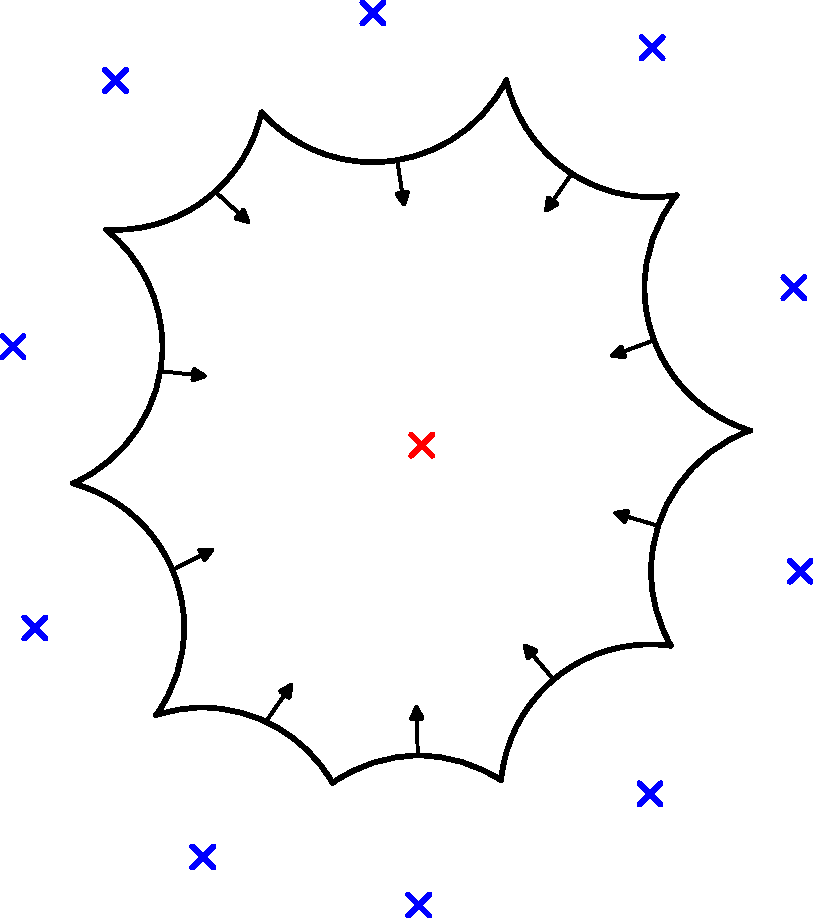
\includegraphics[width=\textwidth]{build/WaveContracting.pdf}
        \caption{The measured wave is re-emitted by the receivers and contracts at the source-location}\label{fig:WaveTimeReversalContraction}
    \end{minipage}
\end{figure}
% !TeX root = ../main.tex
% Add the above to each chapter to make compiling the PDF easier in some editors.

\chapter{Background}\label{chapter:background}
In this chapter, the theoretical background of time-reversal imaging and rays as model for electromagnetic waves according to Maxwell's equations is presented.
These two concepts are essential for understanding the the time-reversal imaging process proposed in this thesis and its underlying physical principles. 

\section{Time-reversal of the electromagnetic field}
\subsection{Time-reversal invariance of physical laws}
The evolution of a physical system in time can be described by a curve \(s(t) \in \mathbb{P}\) that is moving inside a state-space \(\mathbb{P}\).
This state-space is a high-dimensional space, where each dimension represents a physical property (e.g.~mass, velocity, kinetic energy etc.) of each component of the system.
It should not be confused with the physical space.

In general the time-reversal transformation consists of two components\parencite{roberts_reversing_2022}.
First, the curve \(s(t)\) has to be time-reversed by \(s(t) \mapsto s(-t)\).
This means, that the sequence of the states is reversed with respect to time.
Secondly, a time-reversal operator has to be applied to each individual instantaneous state \(s(t) \mapsto \mathcal{T}s(t)\), i.g.\ a ball with velocity to the right would become a ball with velocity to the left.
The time-reversal operator acts by either reversing (momentum) or preserving (kinetic energy) the properties.

In summary, time reversing the curve \(s(t)\) results in the curve \(r(t)=\mathcal{T}s(-t)\). 

As mentioned before, the curve \(s(t)\) inside the state-space \(\mathbb{P}\) describes the evolution of a physical system in time.
This means, \(s(t)\) is a solution to the equations given by the laws that describe the system. 
A law being time-reversal invariant, therefore implies that the time-reversed curve \(r(t)\) is also a solution to this law~\parencite{roberts_time_2021}.

For a more hands-on example, imagine filming a ball that is influenced by gravity while flying through a vacuum.
Newtons second law \({F}=m \cdot {a}\) is time-reversal invariant. This means the film can be played backwards and the trajectory of the ball will still follow Newtons second law.
An example for a non time-reversal invariant law is the second law of thermodynamics, which states that the entropy of an isolated system never decreases.
This means, that a film of a gas spreading out in a room played backwards would not comply to this law, as the entropy of the system in the backwards film actually decreases by time.



\subsection{Time-reversal invariance of Maxwell's equations}
Maxwell's equations formulate the foundations of classical electromagnetism.
They relate the electric field \(\bm{E}\), the electric displacement field \(\bm{D}\), the magnetic field \(\bm{H}\) and the magnetic flux density \(\bm{B}\)  by the following equations, where \(\rho \) and \({\bm{J}}\) denote the electric charge and current densities
\begin{align}\label{eq:maxwell}
    \nabla \cdot \bm{D} &= \rho & \nabla \times \bm{E} &= -\frac{\partial \bm{B}}{\partial t} \\
    \nabla \cdot \bm{B} &= 0 & \nabla \times \bm{H} &= \bm{J} + \frac{\partial \bm{D}}{\partial t}
\end{align}
Generally \(\bm{E}\) and \(\bm{D}\) are related by the electric permittivity \(\varepsilon \), while \(\bm{H}\) and \(\bm{B}\) are related by the magnetic permeability \(\mu \).
In this paper only time-invariant, reciprocal and anisotropic media are considered, which means that the permittivity \(\varepsilon \) and the permeability \(\mu \) are hermitian tensors.~\parencite{krowne_electromagnetic_1984}
This leads to a reduced form of Maxwell's equations, where the electric field \(\bm{E}\) and the magnetic field \(\bm{H}\) are related by
\begin{align}\label{eq:maxwell_reciprocal}
    \nabla \cdot (\varepsilon \bm{E}) &= \rho & \nabla \times \bm{E} &= -\mu \frac{\partial \bm{H}}{\partial t} \\
    \nabla \cdot (\mu \bm{H}) &= 0 & \nabla \times \bm{H} &= \bm{J} + \varepsilon \frac{\partial \bm{E}}{\partial t}
\end{align}

For the time-reversal of these equations, one first has to understand, how the time-reversal operator \(\mathcal{T}\) acts on the fields \(\bm{E}\) and \(\bm{H}\).
Taking into account, that the Poynting vector \(\bm{S} = \bm{E} \times \bm{H}\) is a measure for the energy flow of the electromagnetic field, the time-reversal of these fields has to be chosen in a way that the Poynting vector is reversed as well.
This means, that either \(\bm{E}\) or \(\bm{H}\), but not both, have to be reversed so the Poynting vector changes sign. 
According to \parencite{sigwarth_time_2022}, the Maxwell equations remain invariant if the fields and densities are transformed as follows:
\begin{align}
    \mathcal{T}\bm{E} &= \bm{E} & \mathcal{T}\rho &= \rho \\
    \mathcal{T}\bm{H} &= -\bm{H} & \mathcal{T}{\bm{J}} &= -{\bm{J}}
\end{align}

An intuitive but not rigorous explanation for this transformation is given by the fact, that the electric field is a measure for the force acting on a charge, while the magnetic field is a measure for the force acting on a moving charge. 
Accordingly if time is reversed, the direction of the charges will revert and hence the magnetic field should revert. 
In contrast there is no reason for a positive charge to become a negative charge and vice versa, so the electric field stays the same.


With the time-reversal operator defined for all components of Maxwell's equations the time-reversal of the electric and magnetic field in the time domain can now be written as
\begin{equation}
    \bm{E}_{TR}(t) = \bm{E}(-t) \quad \bm{H}_{TR}(t) = -\bm{H}(-t)
\end{equation}
The fourier transformation of these equations with \(\mathcal{F}\{X(t)\} = \hat{X}(\omega) = \int X(t) \cdot e^{i\omega t} \, dt\) leads to
\begin{equation}
    \hat{\bm{E}}_{TR}(\omega) = \hat{\bm{E}}{(\omega)}^* \quad \hat{\bm{H}}_{TR}(\omega) = -\hat{\bm{H}}{(\omega)}^*
\end{equation}
where \(^*\) denotes the complex conjugate. 

As only fields in the frequency domain will be considered in the following, the hat is dropped.



\section{Reciprocity and time-reversal}\label{sec:math_foundations_em_tr}
In \parencite{de_rosny_theory_2010} the mathematical groundwork for the time-reversal of electromagnetic waves has been laid out.
This section won't cover the derivation of their results, but review them as they represent the starting point of mathematical justification for the time-reversal of electromagnetic waves.

\subsection{The six-vector formalism}
The mentioned paper uses two formalisms.
The electric and magnetic field are combined into the  six-vector \(\psi \) which is defined as
\begin{equation}
    \psi(\bm{r}) = \begin{pmatrix}
        \bm{E}(\bm{r}) \\
        i \bm{H}(\bm{r})
    \end{pmatrix}
\end{equation}
and a source vector \(q\) is defined as
\begin{equation}
    q(\bm{r}) = \begin{pmatrix}
        -i \bm{J}(\bm{r}) \\
        m(\bm{r})
    \end{pmatrix}
\end{equation}
with \(\bm{J}\) and \(m\) denoting the electric and magnetic current density vectors.

These vector-distributions are linearly related through the Green's function \(G\) of the system
\begin{equation}
    \psi(\bm{r}) = \int G(\bm{r}, \bm{r}^{\prime}) q(\bm{r}^{\prime}) \, d^3 r^{\prime}
\end{equation}
For improved readability the integral is written in the following way
\begin{equation}
    \int G(\bm{r}, \bm{r}^{\prime}) q(\bm{r}^{\prime}) \, d^3 r^{\prime} = [G(\bm{r}) q]
\end{equation}

The above definitions imply that the time-reversal operator \(\mathcal{T}\) acts on the six-vector and the source vector by complex conjugation.
\begin{align}
    \mathcal{T}\psi &= \psi^* \\
    \mathcal{T}q &= q^*
\end{align}

\subsection{The electromagnetic time-reversal equation}
Under the assumption of a reciprocal environment (\(\varepsilon \) and \(\mu \) are hermitian) the following equation is derived in \parencite{de_rosny_theory_2010}:
\begin{equation}\label{time-reversal-equation}
    \begin{aligned}
    & \underbrace{\oint_{\delta \Gamma} G(\bm{r}^{\prime}, \bm{r})\left(\bm{n}\left(\bm{r}^{\prime}\right) \times\left[G^*\left(\bm{r}^{\prime}\right) q^*\right]\right) d^2 r^{\prime}}_{\psi_S(\bm{r})} \\
    &=\underbrace{[G^*(\bm{r}) q^*] - [G(\bm{r}) q^*]}_{\psi_V(\bm{r})}
    \end{aligned}
\end{equation}
Taking into account that \([G^*(\bm{r}) q^*] = \psi^*(\bm{r}) = \mathcal{T}\psi(\bm{r})\), the left-hand side \(\psi_S(\bm{r})\) can be interpreted as a procedure of four steps:
\begin{enumerate}
    \item Measure the electromagnetic field \(\psi \) at the surface \(\delta \Gamma \).\ (\(\oint_{\delta \Gamma} \ldots  (\ldots \times \psi^*(\bm{r}^{\prime})) d^2 r^{\prime}\))
    \item Time-revere these measurements.\ (\(\psi^*(\bm{r}^{\prime}) = \mathcal{T}\psi(\bm{r}^{\prime})\))
    \item Deduce a source distribution \(q_{TR}\) from these time-reversed measurements on the surface \(\delta \Gamma \) according to the normal vector of the surface.\ (\(q_{TR}(\bm{r}^{\prime}) = \bm{n}(\bm{r}^{\prime}) \times \mathcal{T}\psi(\bm{r}^{\prime})\))
    \item Calculate the electromagnetic field \(\psi_S(\bm{r})\) generated by this source distribution.\ (\(\psi_S(\bm{r}) = \oint_{\delta \Gamma} G(\bm{r}^{\prime}, \bm{r}) q_{TR}(\bm{r}^{\prime})\))
\end{enumerate}
The electromagnetic time-reversal equation~\eqref{time-reversal-equation} then states that this field \(\psi_S(\bm{r})\) is equal to the time-reversed field \(\psi_{TR}(\bm{r}) = [G^*(\bm{r}) q^*]\) minus a diverging field \(A(\bm{r}) = [G(\bm{r}) q^*]\).
\begin{equation}
    \psi_S(\bm{r}) = \psi_{TR}(\bm{r}) - A(\bm{r})
\end{equation}
Further investigation of \(A\) shows that it is equal to the field generated by the time-reversed sources.
As the sources are initially turned off, their time-reversed excitation and thus the field \(A\) eventually goes to zero.

In conclusion \parencite{de_rosny_theory_2010} proves that it is possible to compute or recreate the time-reversed version of an electromagnetic field \(\psi_{TR}\) inside of a medium \(\Gamma \) by measuring the field \(\psi \) at the surface \(\delta \Gamma \), applying the time-reversal operator \(\mathcal{T}\) to these measurements and emitting the resulting sources back into \(\Gamma \).



\section{Time-reversal Imaging}
This section is dedicated to the explanation of how time-reversal is used for imaging.
Imaging is a very broad term and can be applied to many different fields.
In this thesis, the word imaging is always referring to solving the electromagnetic inverse scattering problem by producing an image of a target domain.
Inverse scattering focuses on identifying the characteristics of an unknown scatterer, including its form, location, and material composition, based on the information obtained from measured scattered fields.
Here the focus is on the localization of passive targets, which are scatterers that do not emit any electromagnetic waves themselves.
This problem is closely related to active-source localization, as the scattered field produced by passive targets can be interpreted as the radiated field from an induced source.~\parencite{chen_computational_2018}

\subsection{Active-Source localization}
Assuming that \(N\) point-sources, denoted as \(q_i(\omega)\), are located at positions \(\bm{r_i}\), the source-distribution \(q(\bm{r}, \omega)\) is obtained, with \(\delta(\bm{r}) \) denoting the dirac delta-function.
\begin{equation}
    q(\bm{r}, \omega) = \sum_{i=1}^{N} \delta(\bm{r} - \bm{r_i}) \cdot q_i(\omega)
\end{equation}
To explain how the described time-reversal process can be used for active-source localization, a signal theory approach is taken.
To do this the medium is modelled as a reciprocal LTI-System.
Now the propagation of an electromagnetic wave-signal \(\psi(\bm{r}, \omega )\) from a source \(q_a(\omega )\) at \(\bm{r_a}\) to a receiver at \(\bm{r_b}\) can be reduced to a simple input-output system with the transfer function \(H_{a\rightarrow b}(\omega) = G(\bm{r_a}, \bm{r_b}, \omega)\).
\begin{equation}
    \psi(\bm{r_b}, \omega) = H_{a\rightarrow b}(\omega) \cdot q_a(\omega)
\end{equation}
This can be applied to the whole source distribution \(q(\bm{r}, \omega)\) to obtain the wave-signal at the receiver \(\bm{j}\).
\begin{equation}
    \psi(\bm{r_j}, \omega) = \sum_{i=1}^{N} H_{i\rightarrow j}(\omega) \cdot q_i(\omega)
\end{equation}
From this wave-signal, an equivalent source \(p_j(\omega)\) can be deduced by applying the measurement operator \(\mathcal{M}\). This is done at all \(M\) receivers at the locations \(\bm{r_j}\).  
\begin{equation}
    p_j(\omega) = \mathcal{M} \psi(\bm{r_j}, \omega)
\end{equation}
Time-reversing (complex-conjugating) the measured sources at all the receivers and remitting them will result in the wave-signal distribution \(\psi_{TR}(\bm{r_x}, \omega)\) which is again measured with \(\mathcal{M}\)
\begin{equation}\label{signal-time-reversal}
    \mathcal{M} \psi_{TR}(\bm{r_x}, \omega) = \sum_{j=1}^{M} \mathcal{M} H_{j\rightarrow x}(\omega ) \cdot p_j^*(\omega) = \sum_{j=1}^{M} \sum_{i=1}^{N} \mathcal{M} H_{j\rightarrow x}(\omega) \cdot \mathcal{M}^* \bm{H}^*_{i\rightarrow j}(\omega) \cdot q^*_i(\omega)
\end{equation}
At this point it should be mentioned, that the usage of \(\psi \), \(q\) and the relating measurement operator \(\mathcal{M}\) was chosen for consistency with Section~\ref{sec:math_foundations_em_tr}.
In most papers about electromagnetic time-reversal only the electric field \(\bm{E}\) is considered for simplicity.
Then, by substituting \(\bm{E}\) for \(\psi \) and describing the sources \(q_i\) by the electric field \(\bm{E}_i\) they cause at location \(\bm{r_i}\) (i.e.~\(\mathcal{M}=1\)), equation~\eqref{signal-time-reversal} becomes
\begin{equation}\label{electric-time-reversal}
    \bm{E}_{TR}(\bm{r_x}, \omega) = \sum_{j=1}^{M} \sum_{i=1}^{N} H_{j\rightarrow x}(\omega )  \bm{H}^*_{i\rightarrow j}(\omega) \cdot \bm{E}^*_i(\omega)
\end{equation}
This approach is valid if the receivers are located in the far-field of the sources.
Here the electric and magnetic fields are orthogonal, so it is sufficient to only keep track of the electric field.
Furthermore the deduction of an equivalent source \(q_{TR}(\bm{r}) = n(\bm{r}) \times \psi^*(\bm{r})\) can be simplified so the electric and magnetic current densities are proportional to the electric and magnetic field respectively~\parencite{de_rosny_theory_2010}
\begin{equation}
    q_{T R}(\bm{r})= \begin{pmatrix}
        -i \bm{J}^*(\bm{r}) \\
        m^*(\bm{r})
    \end{pmatrix} =\left(\begin{array}{c}
        \frac{i \bm{E}^*(\bm{r})}{\eta} \\
        \eta \bm{H}^*(\bm{r})
        \end{array}\right)
\end{equation}
At any source location \(\bm{r_k}\) equation~\eqref{electric-time-reversal} becomes
\begin{equation}\label{electric-time-reversal-source}
    \bm{E}_{TR}(\bm{r_k}, \omega) = \underbrace{\sum_{j=1}^{M} H_{j\rightarrow k}(\omega) \bm{H}^*_{k\rightarrow j}(\omega) \cdot \bm{E}^*_k(\omega)}_{\text{Constructive}} + \underbrace{\sum_{\substack{i=1 \\ i \neq k}}^{M} \sum_{i=1}^{N} H_{j\rightarrow x}(\omega ) \bm{H}^*_{i\rightarrow j}(\omega) \cdot \bm{E}^*_i(\omega)}_{\text{Destructive}}
\end{equation}
As mentioned before, the system is reciprocal so \(H_{j\rightarrow k}(\omega )= H_{k\rightarrow j}(\omega )\). 
Therefore the Constructive part is equal to \(|H_k(\omega)|^2 \cdot \bm{E}^*_k(\omega)\), with
\begin{equation}
    |H_k(\omega)|^2 = \sum_{j=1}^{M} |H_{j\rightarrow k}(\omega)|^2
\end{equation}
This means the constructive part reconstructs the time-reversed signal at the source location \(\bm{r_k}\) without any phase distortion (\(\Im \{{|H_k(\omega)|^2}\} = 0\)) and an attenuation factor of \(|H_k(\omega)|^2\).
Conversely the Destructive part is the sum of all cross-terms of the transfer functions \(H_{j\rightarrow k}(\omega)\) and \(H_{i\rightarrow j}(\omega)\) with \(i \neq k\) that will eventually cancel each other out if the number of receivers goes to infinity.

If~\eqref{electric-time-reversal} is evaluated at any non-source location, no Constructive part will arise, hence the time-reversed signal at this location approaches zero.
With this in mind one can see how equation~\eqref{electric-time-reversal} approximates the time-reversed active-source distribution. 
\begin{equation}
    \bm{E}_{TR}(\bm{r}, \omega) \approx \bm{E}_{TR-source}(\bm{r}, \omega) =  \sum_{i=1}^{N} \delta(\bm{r}-\bm{r_i}) \cdot \bm{E}^*_i(\omega)
\end{equation}

\subsection{Monochromatic signals}
Although there are quite promising attempts of improving the imaging from the reconstructed time-reversed field by using time-domain techniques, like a correlation-based criteria~\parencite{li_correlation-based_2021}, the focus of this thesis will remain on the frequency-domain using monochromatic signals.
These are defined by their amplitude \(|\bm{E}|\) and phase \(\phi \) at a single frequency \(\omega \) and are usually described by a complex pointer \(\underline{\bm{E}}(\bm{r})\).
\begin{equation}
    \underline{\bm{E}}(\bm{r}) = |\bm{E}(\bm{r})| \cdot e^{i \phi(\bm{r})} = |\bm{E}(\bm{r})| \cdot (\cos(\phi(\bm{r})) + i \sin(\phi(\bm{r})))
\end{equation}
The time-domain representation of the signal at location \(\bm{r}\) is retrieved by taking the real part of the product of the pointer and \(e^{i \omega t}\).
\begin{equation}
    \bm{E}(\bm{r}, t) = \Re \{\underline{\bm{E}}(\bm{r}) \cdot e^{i \omega t}\} = |\bm{E}(\bm{r})| \cdot \cos(\phi(\bm{r}) + \omega t)
\end{equation}
For the pointer \(\underline{\bm{E}}(\bm{r})\) the time-reversal operator \(\mathcal{T}\) is simply a reflection along the real axis or (in mathematical terms) a negation of the phase.

The propagation of a monochromatic wave-signal along a straight line through a system can be modelled by the pointer rotating counter-clockwise in the complex plane.
How far the pointer is rotated is given by the phase of the system's transfer function \(\bm{H}(\bm{r_{source}}, \bm{r})\).
Reflecting the pointer along the real axis will result in the same pointer as if the initial pointer was rotated clockwise while propagating through the system.
This means the time-reversal procedure for monochromatic-signals consists simply of rotating the pointer back along the path it took.
This way all the measured pointers at the receivers rotated back will align in the source-location and hence interfere constructively, resulting in a maximum of amplitude at this point.  

\vspace{1cm}
In conclusion, measuring the far field with multiple sensors and subsequently calculating the field that would be created by antennas at the measurement locations emitting the time-reversed signal will result in an amplitude distribution that is maximal at the source locations.
This will then enable the localization of the sources. 
The corresponding imaging formula for \(N\) measurements \(E_i\) of monochromatic waves of frequency \(\omega \) at the locations \(\bm{r_i}\) as presented in~\parencite{peng_zhang_comparison_2013} is
\begin{equation}
    I^{\mathrm{TR}}\left(r_p\right)=\sum_{i=1}^N E_{i}^* \cdot G\left(r_i, r_p, \omega\right)
\end{equation}
In this formula \(G(r_i, r_p, \omega) = H_{i\rightarrow p}(\omega)\) represents the propagation of the wave from the source \(i\) to the imaging-point \(p\).



\section{The Ray Concept of Electromagnetic waves}
To calculate the imaging formula one needs to know the transfer-function \(H_{i\rightarrow p}(\omega)\) between every receiver and every imaging-point in the target-domain.
This could be done by full-wave simulations of delta-impulses at the measurement locations.
These simulations are extremely computationally expensive.
For this reason a geometric ray-tracing approach is taken to calculate these channel characteristics.
The following section will discuss the connection between Maxwell's equations and geometrical optics, to justify the use of rays for the calculation of the transfer-function, if the wavelength \(\lambda \sim \omega^{-1} \) is small enough.

\subsection{Deriving the Eikonal equation from Maxwell's equations}
The following argumentation is based on~\parencite{born_geometrische_1933} and~\parencite{sommerfeld_anwendung_1911}.

Consider a source-free (\(q(\bm{r}) = \bm{J}(\bm{r}) = 0\)) and isotropic (\(\varepsilon(\bm{r}) = \varepsilon_0 \cdot \varepsilon_r(\bm{r})\) and \(\mu(\bm{r}) = \mu_0 \cdot \mu_r(\bm{r}) \)) medium with no free charges (\(\nabla \cdot \bm{E} = 0\)).
Maxwell's equations can then be further simplified to
\begin{align}
    \nabla \cdot \bm{E} &= 0 & \nabla \times \bm{E} &= -\mu \frac{\partial \bm{H}}{\partial t}\label{electric_curl} \\
    \nabla \cdot \bm{H} &= 0 & \nabla \times \bm{H} &= \varepsilon \frac{\partial \bm{E}}{\partial t}\label{magnetic_curl}
\end{align}
Taking the curl of equation~\eqref{electric_curl} and differentiating~\eqref{magnetic_curl} with respect to time yields
\begin{align}
    \nabla \times (\nabla \times \bm{E}) &= -\mu (\frac{\partial}{\partial t} \nabla \times \bm{H}) \\
    \frac{\partial}{\partial t} \nabla \times \bm{H} &= \varepsilon \frac{\partial}{\partial t^2} \bm{E}
\end{align}
Substituting the second equation into the first one results in
\begin{equation}
    \nabla \times (\nabla \times \bm{E}) = \mu \varepsilon \frac{\partial^2}{\partial t^2} \bm{E}
\end{equation}
Finally, using Green's vector identity (\(\nabla \times (\nabla \times A) = \nabla(\nabla \cdot A) - \nabla^2 A\)) the wave equation for the electric field is obtained, where \(\nabla^2\) denotes the componential Laplacian operator.
\begin{equation}
    \nabla^2 \bm{E} + \mu \varepsilon \frac{\partial^2}{\partial t^2} \bm{E} = 0
\end{equation}
The same equation can be derived for the magnetic field and holds for each single component \(\phi \) of both fields.
For monochromatic waves of frequency \(\omega \) it can be written in the frequency domain as
\begin{equation}\label{electromagnetic_wave_equation}
    \nabla^2 \phi(\bm{r}) - k_0^2\ n{(\bm{r})}^2 \cdot \phi(\bm{r}) = 0
\end{equation}
with \(k_0 = \omega \sqrt{\mu_0 \varepsilon_0} \) denoting the vacuum wave-number and \(n(\bm{r}) = \sqrt{\varepsilon_r(\bm{r}) \mu_r(\bm{r})}\) denoting the refractive index of the medium.

For a monochromatic wave of frequency \(\omega \) the components \(\phi(\bm{r})\) can be described by the complex pointer \(\underline{\phi}(\bm{r}) = A(\bm{r}) \cdot e^{i k_0 \cdot \psi(\bm{r})}\) with amplitude \(A(\bm{r})\) and phase \(k_0 \cdot \psi(\bm{r})\).
Equation~\eqref{electromagnetic_wave_equation} then converts to 
\begin{equation}\label{electromagnetic_wave_equation_complex}
    \nabla^2 A(\bm{r}) + 2ik_0 \cdot \nabla A(\bm{r}) \nabla \psi(\bm{r}) + k_0^2 A(\bm{r}) \cdot ({n(\bm{r})}^2 - {(\nabla \psi(\bm{r}))}^2) = 0
\end{equation}
with a more detailed derivation in~\ref{derivation}

The transition from physical waves to geometrical optics is marked by the limit of \(k_0 \sim  \lambda^{-1} \rightarrow \infty \).
Dividing~\eqref{electromagnetic_wave_equation_complex} by \(k_0^2 A(\bm{r})\) and assuming that the amplitude is slowly varying, the limit \(k_0 \rightarrow \infty \) yields the Eikonal equation.
\begin{equation}
    {n(\bm{r})}^2 - {(\nabla \psi(\bm{r}))}^2 = 0 \quad \Leftrightarrow \quad n(\bm{r}) = |\nabla \psi(\bm{r})|
\end{equation}


\subsection{Differential equation of rays}
Wavefronts are surfaces of constant phase \(\psi(\bm{r})\).
Rays are defined as the orthogonal trajectories of the wavefronts and can be written as curves
\begin{equation}
    \bm{r}(l) = \bm{r}_0 + \int_{0}^{l} \bm{v}(\bm{r}(l^{\prime})) \, dl^{\prime}
\end{equation}
with the unit-ray-vector \(\bm{v}(\bm{r}) = \frac{\nabla \psi(\bm{r})}{|\nabla \psi(\bm{r})|}\).


The Eikonal equation combined with the unit-ray-vector leads to the differential equation of rays.
\begin{equation}\label{ray-differential-equation}
    n(\bm{r}) \cdot \bm{v}(\bm{r}) = \nabla \psi(\bm{r})
\end{equation}
Considering the identities \(\nabla(A^2)= 2 \cdot A \cdot \nabla A\) and \(\nabla[{(\nabla A)}^2] = 2 \cdot \nabla A \cdot \nabla^2 A\) and deriving equation~\eqref{ray-differential-equation} with respect to \(l\) yields~\parencite{born_foundations_1999}
\begin{align}
    \frac{d}{dl}(n(\bm{r}) \cdot \bm{v}(\bm{r})) &= \frac{d}{dl}(\nabla \psi(\bm{r})) = \nabla^2 \psi(\bm{r}) \cdot \frac{d\bm{r}}{dl} \\
    &= \nabla^2 \psi(\bm{r}) \cdot \bm{v}(\bm{r}) = \nabla^2 \psi(\bm{r}) \cdot \nabla \psi(\bm{r}) \cdot \frac{1}{n(\bm{r})} \\
    &= \frac{1}{2n(\bm{r})} \cdot \nabla[{(\nabla \psi)}^2] = \frac{1}{2n(\bm{r})} \cdot \nabla({n(\bm{r})}^2) \\
    &= \nabla n(\bm{r})
\end{align}
For a ray in a homogenous medium, i.e.~\(n(\bm{r}) = n_0\), this equation becomes
\begin{equation}
    n_0 \cdot \frac{d}{dl}\bm{v}(\bm{r}) = 0
\end{equation}
so the unit-ray-vector is a constant and hence the ray is a straight line.
\begin{equation}
    \bm{r}(l) = \bm{r}_0 + l \cdot \bm{v}_0
\end{equation}


\subsection{Refraction and Reflection at plane interfaces}
At a plane interface \(\Gamma \) of two homogenous media (\(\Lambda_1\) and \(\Lambda_2\)) with different refractive indices \(n_1\) and \(n_2\), the differential equation of rays must be fulfilled.
An incident ray with unit-vector \(\bm{v}_1\) and the transmitted ray with unit-vector \(\bm{v}_2\) therefore satisfy the following conditions at any point on the interface.
\begin{equation}
    n_1 \cdot \bm{v}_1 = \nabla \psi|_{r \in \Lambda_1 } \quad n_2 \cdot \bm{v}_2 = \nabla \psi|_{r \in \Lambda_2 } 
\end{equation}
The closed integral over a gradient field is always zero.
For any rectangular curve \(C\) (width \(w\) and height \(h\)) where the edges of length \(w\) are tangential to \(\Gamma \) the integral of the gradient field must still be zero.
The tangential parts of the curve are either in \(\Lambda_1\) or \(\Lambda_2\).
Taking the limit of \(h \to 0\) then results in~\parencite{born_foundations_1999}
\begin{equation}
    \lim_{h \to 0} \oint_C \nabla \psi \cdot d\bm{r} = \int_{0}^{w} \nabla \psi|_{r \in \Lambda_1 } \cdot \bm{t} \, dw' + \int_{0}^{w} \nabla \psi|_{r \in \Lambda_2 } \cdot (-\bm{t}) \, dw' = 0
\end{equation}
This means that the tangential components of the ray-vectors \(n \cdot \bm{v}\) are continuous across the interface.
\begin{equation}
    (n_2 \bm{v}_2 - n_1 \bm{v}_1) \cdot \bm{t} = 0
\end{equation}
With \(\bm{t} = \bm{b} \times \bm{n}\) where \(\bm{n}\) is the normal vector of \(\Gamma \) and \(\bm{b}\) is the normal vector of the plane where \(C\) lies this becomes
\begin{equation}
    \bm{b} \cdot [\bm{n} \times (n_2 \bm{v}_2 - n_1 \bm{v}_1)] = 0
\end{equation}
This equation holds for an arbitrary orientation of the curve \(C\) as long as the edges of length \(w\) are completely in either \(\Lambda_1\) or \(\Lambda_2\).
This implies that \(\bm{b}\) can be chosen arbitrarily as long as \(\bm{t} = \bm{b} \times \bm{n}\) still holds.
With this in mind and \(\theta_1\),\(\theta_2\) denoting the angles of \(\bm{v}_1\),\(\bm{v}_2\) with the surface normal \(\bm{n}\), Snell's law is retrieved
\begin{equation}
    \bm{n} \times (n_2\bm{v}_2) - \bm{n} \times (n_1\bm{v}_1) = 0 \quad \Rightarrow \quad n_1 \sin(\theta_1) = n_2 \sin(\theta_2)
\end{equation}

It is known, that at the transition between two media with different refractive indices there is always a refracted as well as a reflected wave.
The reflected wave is in the same medium as the incident wave, which leads to the law of specular reflection.
\begin{equation}
    \sin(\theta_{inc}) = \sin(\theta_{ref})
\end{equation}


\subsection{Phase and Amplitude propagation along ray-paths}
According to the definition of the ray-path \(\bm{r}(l)\) and the Eikonal equation, the derivation of the phase \(k_0 \cdot \psi(\bm{r})\) of a wave along this path is always equal to \(k_0\) times the refractive index \(n(\bm{r})\) so the phase propagation can be written as
\begin{equation}
    k_0 \cdot \psi(\bm{r}(l)) = k_0 \cdot \int_{0}^{l} n(\bm{r}(l^{\prime})) \, dl^{\prime}
\end{equation}
In a homogenous medium this simplifies to
\begin{equation}
    k_0 \cdot \psi(\bm{r}(l)) = k_0 \cdot n \cdot l
\end{equation}

The Amplitude on the other hand has a much more complex behavior even along ray-paths.
For a single point-source in a lossless medium the radiated energy is conserved so the integral over the Poynting-Vector \(S\) over a sphere \(\mathcal{S} \) of radius \(r\) must be independent of \(r\).
\begin{equation}
    \int_\mathcal{S}  S \cdot \bm{n} \, d\Omega = |S| \cdot 4\pi r^2 = \text{const}
\end{equation}
This means, the amplitude of \(S\) is inversely proportional to the square of the distance from the source.
The amplitude of the Poynting-Vector is furthermore proportional to the amplitude of the electric field squared, which concludes that the amplitude of the electric field is inversely proportional to the distance from the source.
\begin{equation}
    |\bm{E}| \propto \frac{1}{r}
\end{equation}
In scenarios like the reflection at interfaces, the amplitude and direction of the electric field vector can be calculated by the Fresnel equations, where the polarization of the field is considered as well.
For our case it is sufficient to model a reflective surface with a virtual source that is placed in the mirrored position of the original source with respect to the surface, so the reflected ray's amplitude keeps decreasing with \(\frac{1}{l}\), where \(l\) is the distance from the virtual source.
If the scenario is even more complex, for example curved reflective surfaces, or sharp edges, a more sophisticated model would be needed.

With these considerations in mind, the propagation of the electric field along a straight ray-path \(\bm{r}(l)\) from a source \(E_0\) through a homogenous medium (refractive index \(n\)), with \(l\) denoting the distance from the source, can be described as
\begin{equation}
    \underline{\bm{E}}(l) = \frac{1}{l} \cdot E_0 \cdot e^{i k_0 \cdot n \cdot l}
\end{equation}




\subsubsection{Derivation}\label{derivation}

Consider these identities
\begin{align}
    \nabla^2 (a \cdot b) &= \nabla^2 a \cdot b + 2 (\nabla a \nabla b) + a \nabla^2 b, \\
    \nabla e^{i k_0 \cdot \psi(\bm{r})} &= i k_0 \cdot \nabla \psi(\bm{r}) \cdot e^{i k_0 \cdot \psi(\bm{r})}, \\
    \nabla^2 e^{i k_0 \cdot \psi(\bm{r})} &= - k_0^2 \cdot {(\nabla \psi(\bm{r}))}^2 \cdot e^{i k_0 \cdot \psi(\bm{r})}.
\end{align}
which lead to
\begin{gather}
    \nabla^2 (A(\bm{r}) \cdot e^{ik_0 \cdot \psi(\bm{r})}) \\
    = (\nabla^2 A(\bm{r}) + 2ik_0 \cdot \nabla A(\bm{r}) \nabla \psi(\bm{r}) - k_0^2 \cdot (\nabla \psi(\bm{r}))) \cdot e^{ik_0 \cdot \psi(\bm{r})}
\end{gather}
This results in the following equivalence (\(\underline{\phi}(\bm{r}) = A(\bm{r}) \cdot e^{ik_0 \cdot \psi(\bm{r})}\))
\begin{gather}
    \nabla^2 \underline{\phi}(\bm{r}) + k_0^2\ n{(\bm{r})}^2 \cdot \underline{\phi}(\bm{r}) \stackrel{!}{=} 0, \\
    \Leftrightarrow \nabla^2 A(\bm{r}) + 2ik_0 \cdot \nabla A(\bm{r}) \nabla \psi(\bm{r}) + k_0^2 A(\bm{r}) \cdot ({n(\bm{r})}^2 - {(\nabla \psi(\bm{r}))}^2) \stackrel{!}{=} 0.
\end{gather}
% !TeX root = ../main.tex
% Add the above to each chapter to make compiling the PDF easier in some editors.

\chapter{The Ray Tracing Approach}\label{chapter:the_raytracing_approach}
In Chapter~\ref{chapter:background} the theoretical background for time-reversal imaging and the utilization of ray tracing for the needed wave-simulation were laid out.
This chapter will describe the implementation of a ray tracing approach for the time-reversal imaging algorithm.

As mentioned in \parencite{dyab_critical_2013} the quality of the time-reversed image increases within a highly reverberant environment.
In contrast to other imaging algorithms, multipath propagation of the waves is therefore not suppressed but used to improve the time-reversal imaging.
To simulate the multipath propagation, one is interested in all the paths that the signal takes from the source to the imaging domain.
The multipath propagation is mostly caused by reflections and refractions which can be described by the laws of geometrical optics as shown in Section~\ref{sec:ray-concept}.
This is why ray tracing is such a suitable approach for this problem.

\section{The Imaging Algorithm}
The time-reversal imaging algorithm is a three-step process.
First, the scene is illuminated with a monochromatic signal of frequency \(\omega_i\) and the resulting scattered field is recorded at \(M\) receiver locations \(\bm{r}_j\). 
This step is repeated for \(N\) frequencies \(\omega_i\) resulting in the \(N \times M\) matrix \(\mathsf{E} \) containing the scattered field at all receiver locations for all frequencies.

In the second step, a random location in the target domain is chosen as the source of a big number of rays (\(N_{\text{rays}}\approx 10^{9}\)) which are launched into equally distributed random directions.
A ray that follows a possible path from the target location to a receiver location will eventually hit the receiver so the path can be recorded.
From these paths, the paths for the other locations in the target domain can be derived by using virtual targets as described in Section~\ref{section:virtual_targets}.
This step is necessary because shooting \(N_{\text{rays}}\) rays in all directions from all points in the target domain would be computationally expensive.

The virtual targets resulting from the second step are then grouped into wavefronts, which are further described in Section~\ref{section:subdivision_into_wavefronts}.
Finally, the field contribution of each wavefront at any point in the imaging domain is calculated.
The measured scattered field \(\underline{\mathsf{E}}\) is complex conjugated and sent back from every corresponding receiver to all points in the imaging domain along the paths of this wavefront.
The calculation of the field propagation along this ray-path from one hit-point to the next is described in Section~\ref{section:calculation_of_the_field_propagation}.

The sum of all receiver contributions at each point in the imaging domain then gives rise to the time-reversed field of this wavefront in the imaging domain.
By taking the absolute value of the time-reversed field, the image is obtained.
For a better resolution of the image, this step is repeated for all measured frequencies \(\omega_i\).
This can be summarized in the imaging formula of the n-th wavefront
\begin{equation}
    I_n(\bm{r}_k) = |\sum_{i=1}^{N} \sum_{j=1}^{M} \underline{\mathsf{E}}_{ij}^* \cdot H_{j \rightarrow k}(\omega_i)|
\end{equation}
where \(H_{j \rightarrow k}(\omega_i)\) is the transfer function from receiver \(j\) to point \(k\) in the imaging domain at frequency \(\omega_i\) along the n-th wavefront, which is calculated by tracing the electric field along the ray-path according to~\eqref{eq:field-along-ray-path}.


\section{Implementation of Virtual Targets for Multipath Wave Propagation}\label{section:virtual_targets}

\begin{figure}[ht]
    \centering
    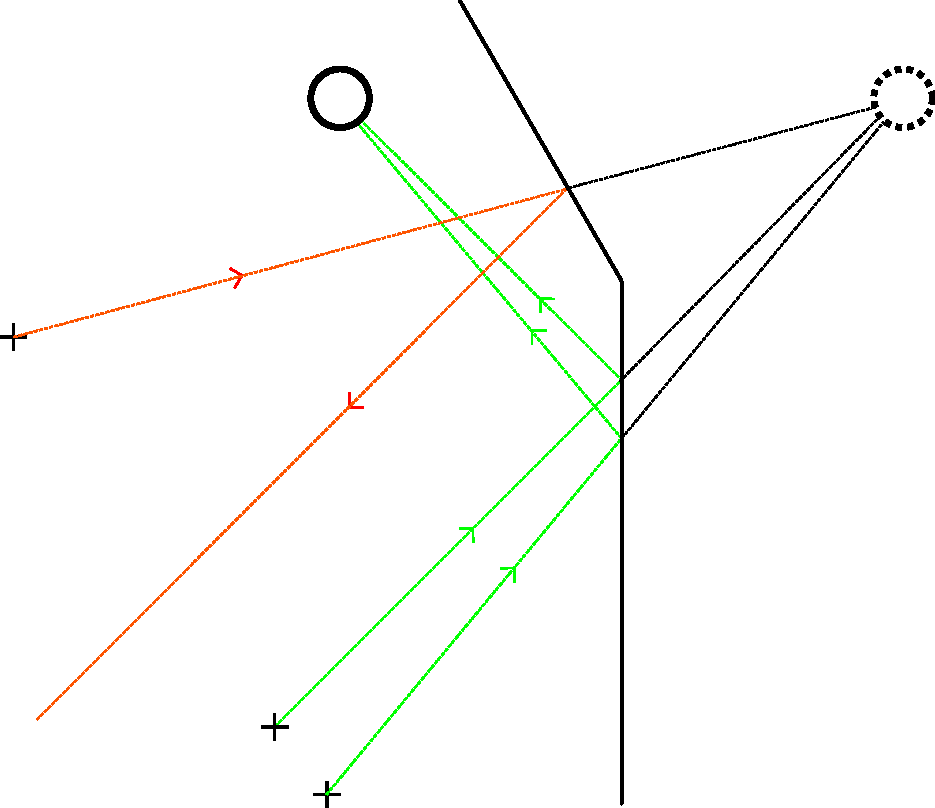
\includegraphics[width=0.5\textwidth]{figures/VirtualTargets.pdf}
    \caption{The green paths show, how shooting a ray at a virtual target (dotted circle) from different locations can result in hitting the original target (full line circle). The red path on the other hand does not hit the target because its launch location is too far away from the other launch locations.}\label{fig:virtual_targets}
\end{figure}

To derive the paths for all points in the imaging domain from the paths of a single point in the imaging domain, the concept of virtual targets is used.
In the following, the initial single point in the imaging domain is called the probe point.

A path is distinguished by its launch location, the receiver where it ends, and the sequence of plane surfaces it encounters between the launch point and the receiver.
The receiver is modelled as a sphere with radius \(r_{\text{rec}}\) around the receiver location.
This radius should be chosen big enough, so the randomly generated rays do not all miss the receiver, but small enough to not overlap with other receivers.
If a ray launched from the probe point \(\bm{r}_p\) with the initial direction \(\bm{u}_{\text{init}}\) hits a receiver, any point \(\bm{p} = \bm{r}_p + s \cdot \bm{u}_{\text{init}}\) can be used to reconstruct the path between the probe point and the receiver in the following time-reversal step.
To do this one simply has to shoot a ray from the probe point in the direction of \(\bm{p}\).

\begin{figure}
    \centering
    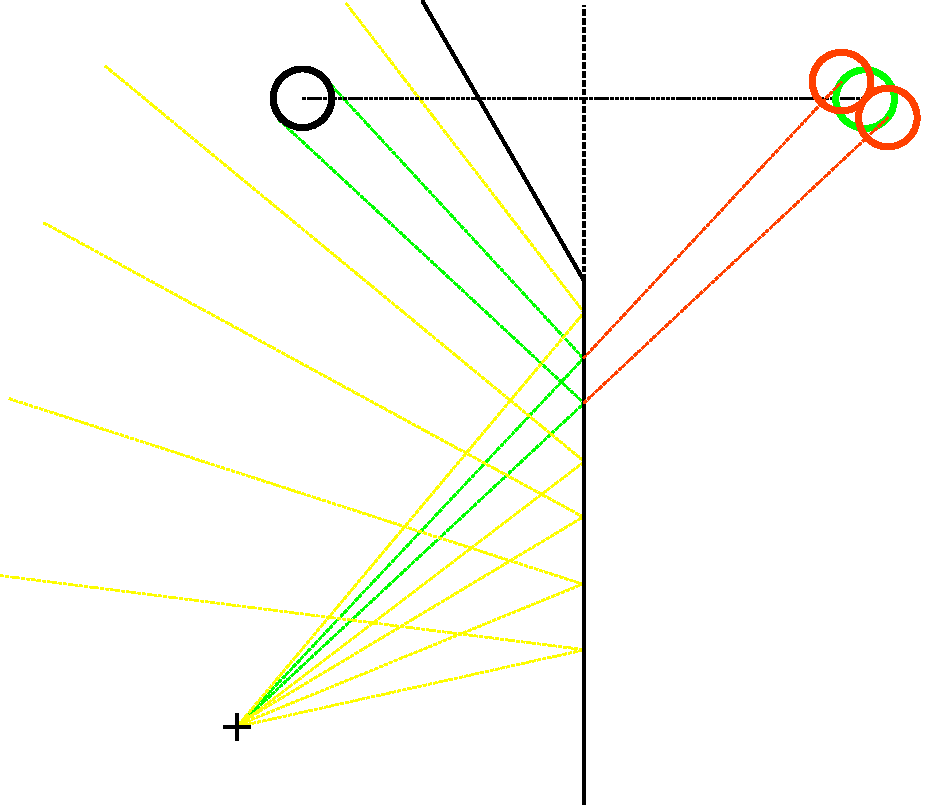
\includegraphics[width=0.5\textwidth]{figures/VirtualTargetsMultiHit.pdf}
    \caption{Two random rays hit the receiver sphere, so two virtual targets would be created (red circles) although there should be only one virtual target (green circle) at the mirrored position of the receiver circle.}\label{fig:mulithit}
\end{figure}

Setting \(s\) to the distance \(d\) that the ray traveled results in the corresponding virtual target \(\bm{v}\).
\begin{equation}\label{eq:visual_target}
    \bm{v} = \bm{r}_p + d \cdot \bm{u}_{\text{init}}
\end{equation}
Shooting a ray from any point \(\bm{r}_k\) close to the probe point in the direction of the virtual target will in most cases hit the same receiver, so the virtual target can be used to reconstruct the path between \(\bm{r}_k\) and the receiver as well  (see Figure~\ref{fig:virtual_targets}).

It is important to stress that this approach only works for points close to the probe point.
If the point is too far away, a ray shot at the virtual target might not hit the receiver.
In a similar way, the virtual targets found for the probe point might not account for all the paths between an imaging point and the receiver.

Another problem arises with this approach when multiple rays with slightly different launch directions hit the same receiver taking the same path (see Figure~\ref{fig:mulithit}).
In this case two virtual targets would be recorded for one actual path.
This would lead to an unwanted increased influence of this path in the time-reversal step.
To resolve this issue, every ray has an associated hash value that is calculated from the path it takes, i.e.~from the object-ID's of the plane surfaces it bounces of and the receiver it finally hits.
This way it can be checked if a virtual target for this path has already been recorded, as every path has an unique hash value.
If this is the case, the new virtual target is not saved.

Furthermore, equation~\eqref{eq:visual_target} is only an approximation of a perfect virtual target, which would be retrieved by mirroring the receiver location at the plane surfaces the ray hits in a backwards manner.
For the sake of simplicity, this is not done in the implementation.
Instead the center of the hit sphere \(\bm{r}_{\text{receiver}}\) is projected on the linear slope of the ray to retrieve a more accurate value for the distance between launch location and receiver along the path.

\begin{equation}
    d_{\text{approx}} = d_{\text{ray\_hit}} +  (\bm{r}_{\text{receiver}} - \bm{r}_{\text{ray\_hit}}) \cdot \bm{u}_{\text{ray\_hit}} \approx d_{\text{actual}}
\end{equation}

\begin{figure}[h]
    \centering
    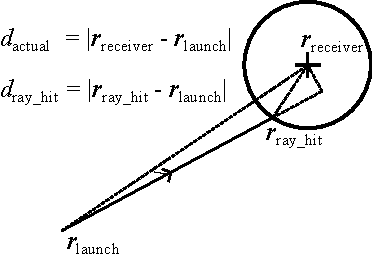
\includegraphics[width=0.5\textwidth]{figures/d_approx.pdf}
    \caption{Projection of \(\bm{r}_{\text{receiver}}\)}\label{fig:d_approx}
\end{figure}


\section{Subdivision Into Wavefronts}\label{section:subdivision_into_wavefronts}
Every virtual target recorded in the preceding step is a version of one of the receivers that was mirrored at the plane surfaces the ray hit.
By shooting rays at them from the imaging domain, the paths between the imaging domain and the receiver locations are reconstructed and therefore the according transfer functions can be simulated.
A subset of virtual targets which accounts for one mirrored version of all receiver locations is called a wavefront.
There are as many wavefronts as there are different paths from one receiver to the probe point.
The virtual targets are mapped to the wavefronts by the hash value of the ray before including the hit receivers object-ID into the hash calculation.
This way, the wavefronts are characterized by the sequence of plane surfaces the rays reflect of.

The term wavefront is used because the paths of the rays to the virtual targets of one wavefront can be seen as the paths of a common wavefront that is emitted from the receiver location.
The subdivision of the virtual targets into wavefronts is done to get more insight into the imaging contribution of each wavefront.
To retrieve the final time-reversed image, the images of all wavefronts simply have to be summed up.


\section{Calculation of the Field Propagation}\label{section:calculation_of_the_field_propagation}
As shown in Equation~\eqref{eq:field-along-ray-path}, the propagation of the electric field along the ray-path according to the path-length \(l\) is calculated by:
\begin{equation}
    \underline{E}(l) = \frac{1}{1 + l} \cdot \underline{E}_0 \cdot \mathrm{e}^{\mathrm{i} k_0 \cdot n \cdot l}
\end{equation} 

The ray tracing program will calculate the location where a ray hits a plane surface (or receiver sphere respectively) and the direction of the reflected ray.
To efficiently trace the field along the ray-path, the resulting field \(\underline{E}_{\text{new}}\) at the hit location should be calculated from the field \(\underline{E}_{\text{old}}\) at the previous hit location (or the launch location respectively), the length of the path at this old hit location \(l_{\text{old}}\) and the distance \(d\) between the old and the new hit point.
\begin{equation}
    \underline{E}_{\text{new}} = \underline{E}_{\text{new}}(l_{\text{new}}) = \underline{E}_{\text{new}}(\underline{E}_{\text{old}}, l_{\text{old}}, d)
\end{equation}
Considering that \(l_{\text{new}} = l_{\text{old}} + d\) the new field can be written as
\begin{equation}
    \underline{E}_{\text{new}} = \frac{1}{1 + l_{\text{old}} + d} \cdot \mathrm{e}^{\mathrm{i} k_0 \cdot n \cdot d}  \cdot \underline{E}_{0} \cdot \mathrm{e}^{\mathrm{i} k_0 \cdot n \cdot l_{\text{old}}} 
\end{equation}
With \(\underline{E}_{\text{old}} = \frac{1}{1 + l_{\text{old}}} \cdot \underline{E}_0 \cdot \mathrm{e}^{\mathrm{i} k_0 \cdot n \cdot l_{\text{old}}} \) the formula for \(\underline{E}_{\text{new}}(\underline{E}_{\text{old}}, l_{\text{old}}, d)\) is retrieved:
\begin{equation}
    \underline{E}_{\text{new}}(\underline{E}_{\text{old}}, l_{\text{old}}, d) = \underline{E}_{\text{old}} \cdot \frac{1 + l_{\text{old}}}{1 + l_{\text{old}} + d} \cdot \mathrm{e}^{\mathrm{i} k_0 \cdot n \cdot d}
\end{equation}

% !TeX root = ../main.tex
% Add the above to each chapter to make compiling the PDF easier in some editors.

\chapter{Results}\label{chapter:results}
The proposed imaging algorithm is tested in various scenarios to evaluate its performance.
To quantify the performance of the algorithm, the quality of the reconstructed images and the needed computational time is evaluated.


The scenarios are categorized into pure Line-of-Sight (LOS), pure Non-Line-of-Sight (NLOS) and mixed scenarios.
As real-world measurements are not feasible for this thesis, the measurement data is generated by the wave simulation program `Altair Feko' using the Method of Moments (MoM).
The imaging domain (red) is defined as the set of 256\(\times \)256 linearly distributed points in the x-y-plane.
Multiple active source-dipoles (blue) are placed in the imaging domain and their scattered field is recorded at 10000 receiver locations (green) in the y-z-plane for 20 logarithmically spaced frequencies between 4.8GHz and 7.2GHz.
This general setup is used for all scenarios as visualized in Figure~\ref{fig:general_setup}.

\begin{figure}[ht]
    \centering
    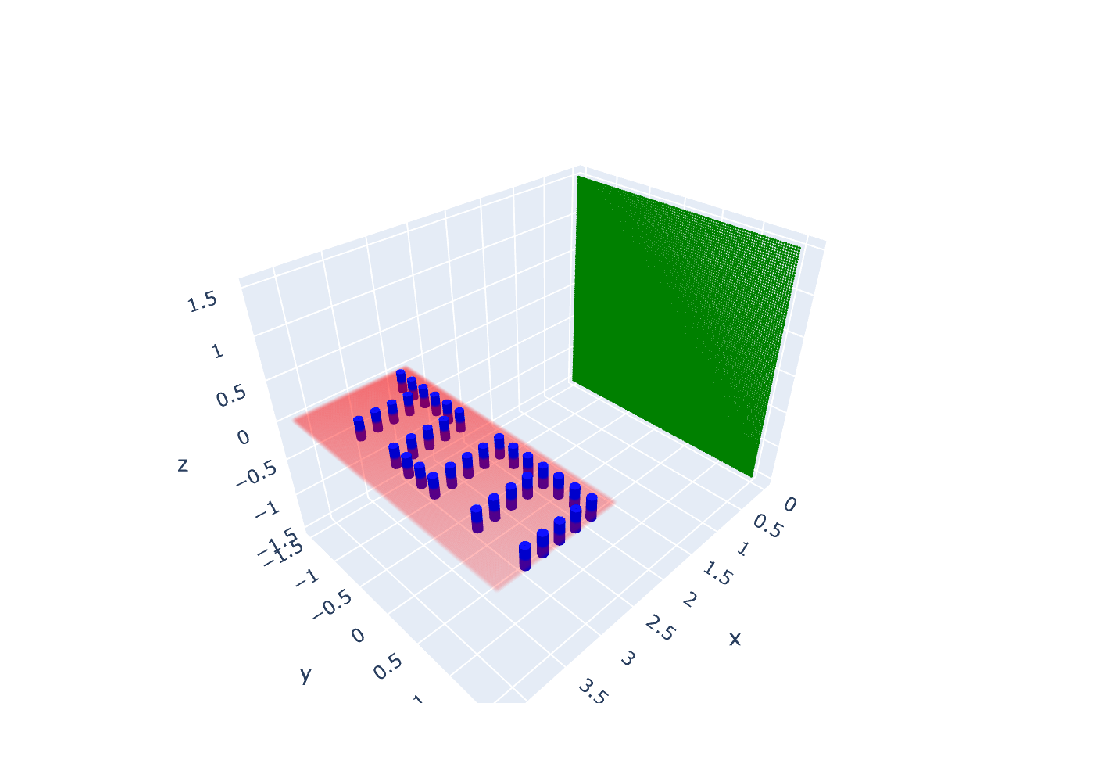
\includegraphics[width=0.8\textwidth]{figures/general_setup.pdf}
    \caption{The General Setup}\label{fig:general_setup}
\end{figure}


The imaging algorithm is then applied to the recorded data to reconstruct the sources in the imaging domain.


\section{Pure Line-of-Sight (LOS) Scenarios}
Pure Line-of-Sight scenarios are the simplest case for the imaging algorithm.
The setup for this scenario is exactly as shown in Figure~\ref{fig:general_setup}.
The source and the receiver are in direct line of sight, so there is only one wavefront that travels from the receivers to the imaging domain without any reflections.
If there are furthermore no refractions (homogenous medium with refractive index \(n\)), the algorithm boils down to the following formula:
\begin{equation}\label{eq:naive_algorithm}
    I(\bm{r}_k) = |\sum_{i=1}^{N} \sum_{j=1}^{M} \frac{\underline{\mathsf{E}}_{ij}^*}{|\bm{r}_j - \bm{r}_k|} \cdot \mathrm{e}^{\mathrm{i}k_0\cdot n \cdot |\bm{r}_j - \bm{r}_k|}|
\end{equation}

\begin{figure}[ht]
    \centering
    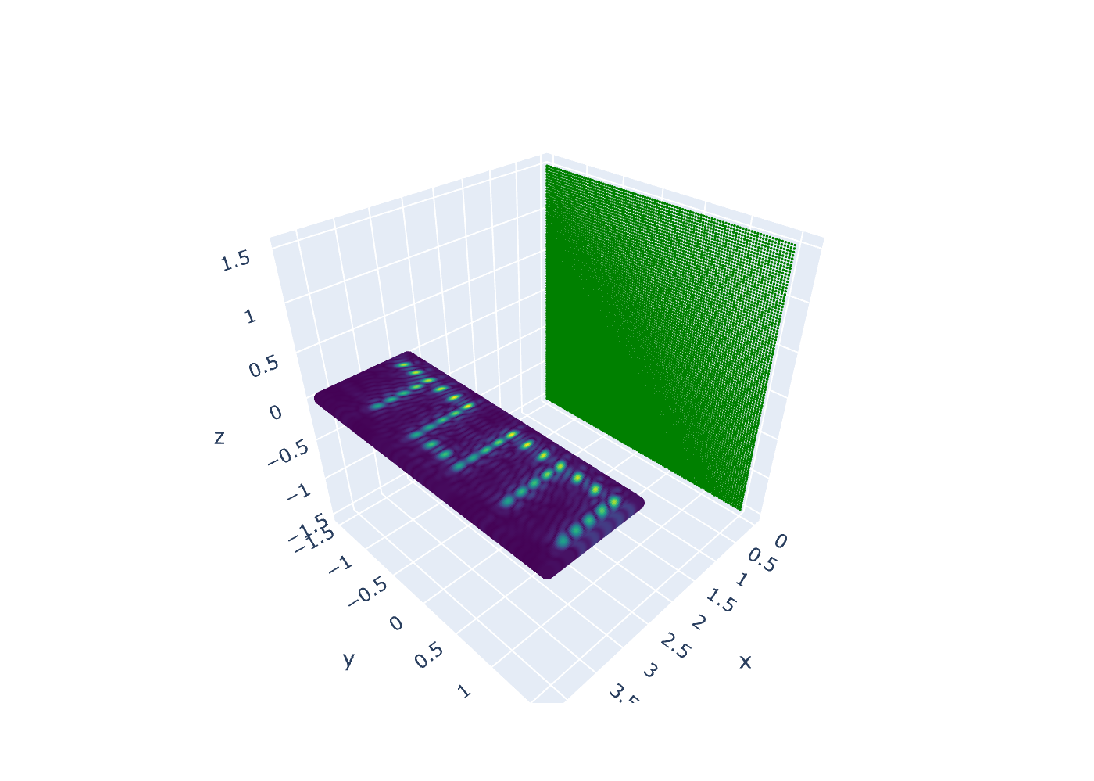
\includegraphics[width=0.8\textwidth]{figures/los_result.pdf}
    \caption{The image of the pure LOS-scenario}\label{fig:los_results}
\end{figure}

The calculated image for this scenario is shown in Figure~\ref{fig:los_results}.
The emitting dipole sources can be easily localized.
This image would also result from evaluating Equation~\eqref{eq:naive_algorithm} at every point in the imaging domain and coloring the imaging point accordingly.
To do this no knowledge about the medium or the setup is needed and only the distances between the receivers and the imaging points are considered.
This approach is called the naive algorithm and is used as a reference to compare the proposed algorithm to.


\section{Pure Non-Line-of-Sight (NLOS) Scenarios}
To create a pure Non-Line-of-Sight scenario, a PEC-plate is placed between the source and the receiver to block the direct path.
Another PEC-plate is placed perpendicular on top of the blocking plate with a small gap between both plates to create a reflecting path.
The resulting setup is shown in Figure~\ref{fig:nlos_setup}.

\begin{figure}[ht]
    \centering
    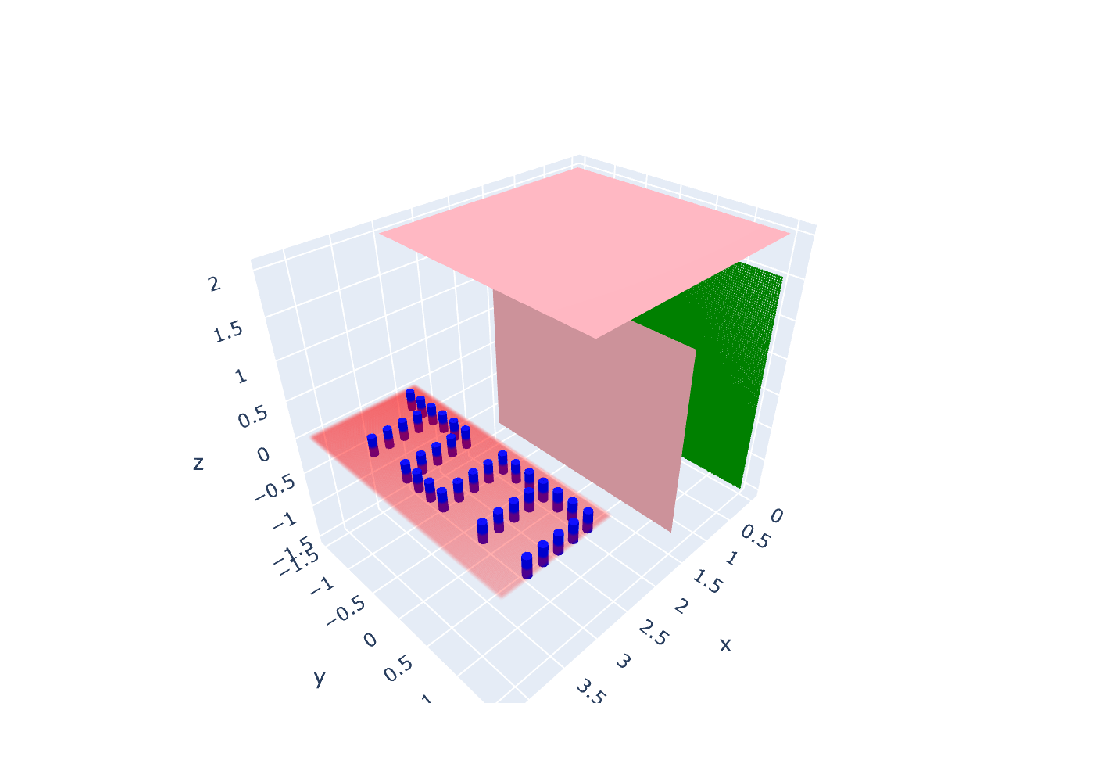
\includegraphics[width=0.8\textwidth]{figures/nlos_setup.pdf}
    \caption{The NLOS Setup}\label{fig:nlos_setup}
\end{figure}

In this setup only a small fraction of the emitted wave will pass through the gap, reflect off the top plate and reach the receivers.
A simpler algorithm that only considers the distances between the receivers and the imaging points would fail to reconstruct the dipole locations.
The proposed algorithm on the other hand is able to reconstruct the sources as shown in Figure~\ref{fig:nlos_results}.
In the plots the paths of the rays that are considered by the algorithm are visualized as yellow lines for some of the imaging points.

\begin{figure}[ht]
    \centering
    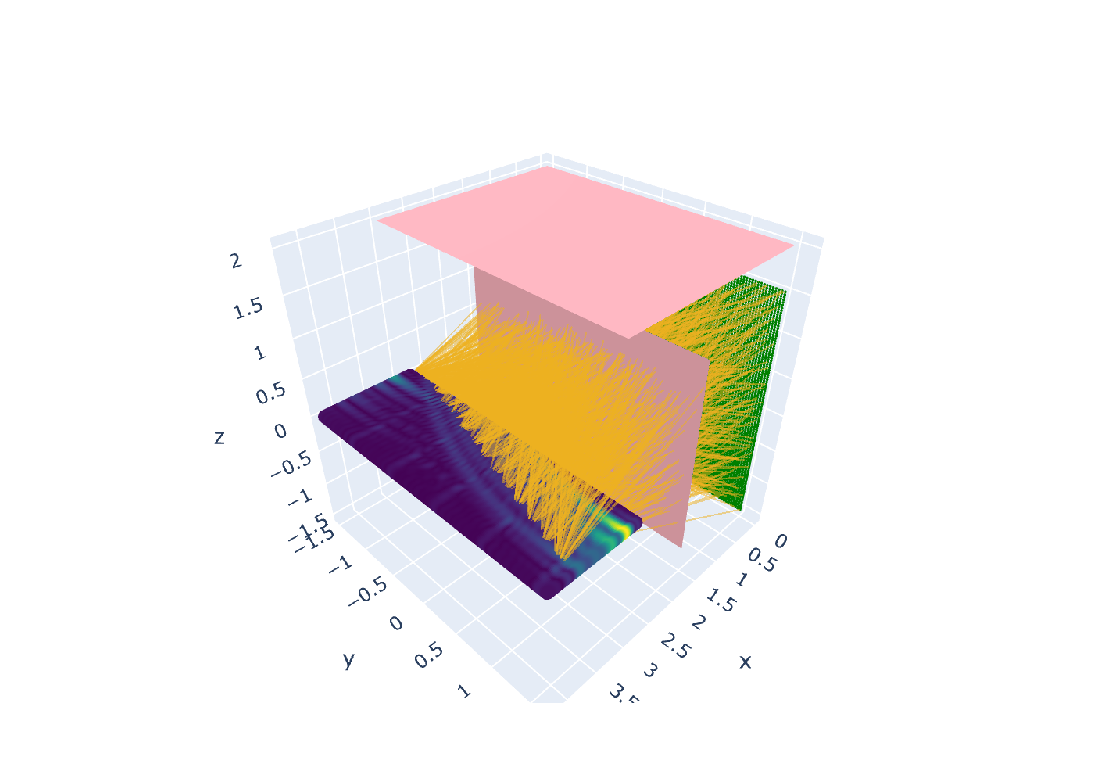
\includegraphics[width=0.49\textwidth]{figures/nlos_naive_result.pdf}
    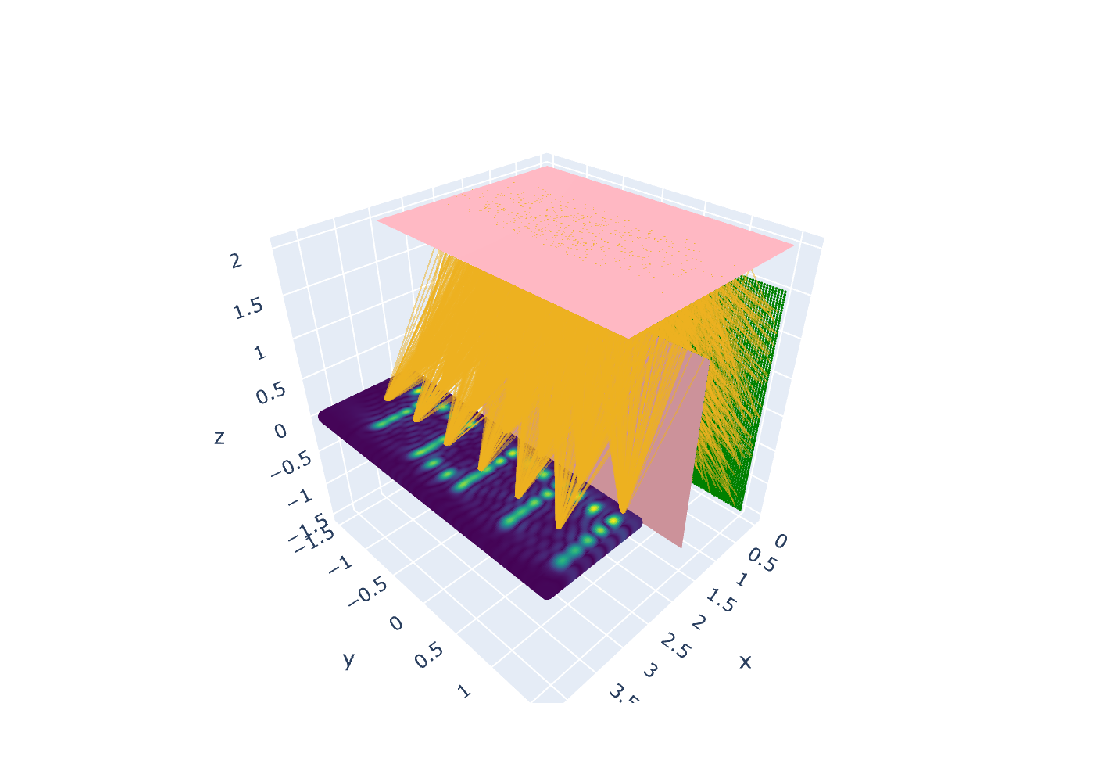
\includegraphics[width=0.49\textwidth]{figures/nlos_result.pdf}
    \caption{The Intensity of the Backpropagated field using a naive algorithm (without considering the PEC-plates) compared to the ray-tracing algorithm}\label{fig:nlos_results}
\end{figure}

This scenario with only one reflection off a plane PEC-plate is very similar to the pure LOS-scenario.
There is no multipath propagation between the source and the receiver, so the algorithm can be simplified to a similar form as Equation~\eqref{eq:naive_algorithm} with the only difference being that the distance between the imaging point and the \textbf{reflected} receiver-location should be considered.



\section{Mixed Scenarios}

\section{Limitations}
% !TeX root = ../main.tex
% Add the above to each chapter to make compiling the PDF easier in some editors.

\chapter{Conclusions and Outlook}\label{chapter:conclusions}
The thesis presented a ray tracing approach for calculating the time-reversal image of a specified domain from measured data in the microwave spectrum.
The needed theoretical background was summarized and the algorithm was tested on a set of different examples.
The results showed that the algorithm is able to improve the image quality by considering the multipath propagation from a surrounding setup, especially when the direct path is blocked.
As greatest advantage of the algorithm the low computational cost was identified.
Through using a GPU for the calculations the algorithm is much faster than a full-wave simulation and can be used for a first approximation of the time-reversal image.
A possible field of further research could be the optimization of the algorithm by improving the placement of the receivers and the reflector plates, so that the number of needed rays can be reduced, while still maintaining a good image quality.
Another possible improvement could be the use of a more sophisticated ray tracing algorithm, that can handle more complex geometries and materials, as in this thesis only plane PEC-plates were used.
Such an algorithm would need to treat the electromagnetic wave as a vector field instead of a simple scalar field, as the polarization of the wave influences the scattering and reflecting process.
Furthermore the performance of the algorithm with real-world measurements could be tested, as the results in this thesis were only based on simulated data.
The algorithm could also be extended to work with other types of waves, like acoustic waves or seismic waves, as the principle of time-reversal imaging is not limited to the microwave spectrum.
The biggest advancement would be made by extending and investigating the algorithm for the localization of passive scatter-points.
For this purpose, the algorithm would also have to consider the locations of illuminating transmitters.





\appendix{}

\microtypesetup{protrusion=false}
\listoffigures{}
\microtypesetup{protrusion=true}

\printbibliography{}

\end{document}
